\documentclass[11pt]{article}
\usepackage[utf8]{inputenc}
\usepackage[spanish,es-tabla]{babel}
\usepackage{amsmath}
\usepackage{amsfonts}
\usepackage{amssymb}
\usepackage{graphicx}

\usepackage{color, colortbl}

\usepackage{hyperref}
\usepackage{float}
\usepackage[a4paper,top=1.5cm,bottom=1.5cm,left=1.5cm,right=1.5cm,marginparwidth=1.75cm]{geometry}

\definecolor{LightYellow}{RGB}{217, 177, 85}

\title{Tubbing S.A \\ \small{Comunicaciones digitales} \\ \small{Universidad Nacional del Comahue} }
\author{ 
        Gatica, Isaias \\ \small{LautaroAndresSaez@gmail.com} \and 
        Millain, Gonzalo \\ \small{gonza.pm@outlook.com} \and
        Saez, Lautaro Andres \\ \small{IsaiasGatica1@gmail.com} 
}

\date{}

\begin{document}
    \maketitle
    \section{Generalidades}
    
        \subsection{Estructuras de redes}
        \begin{figure}[H]
            \centering
            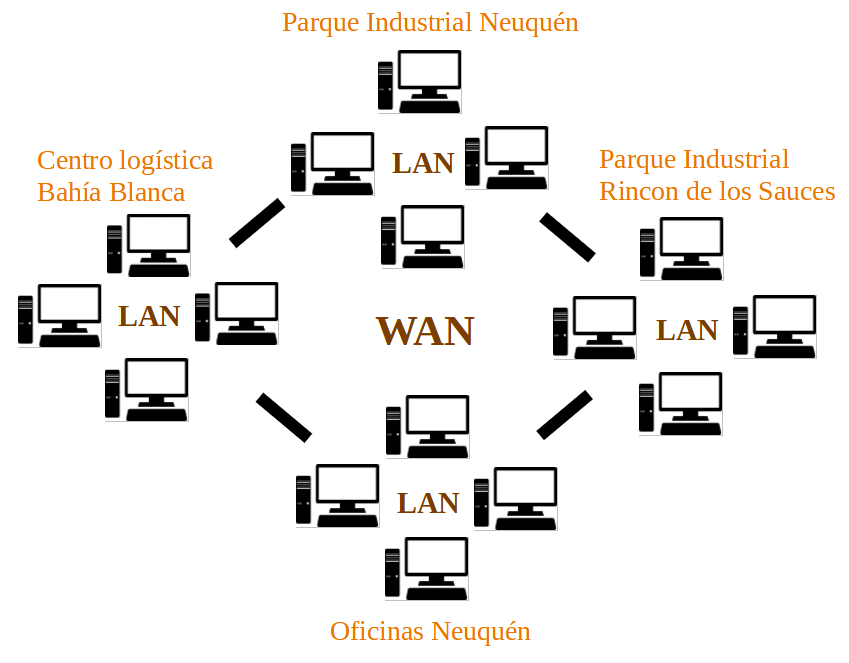
\includegraphics[scale=0.5]{Figure/Tubbin_Estructura.PNG}
            \caption{Imagen representativa de la estructura de Red}
            \label{Estructura}
        \end{figure}


        \subsubsection*{LAN}

        Cada área tendrá su propia red LAN, la cual mas adelante se definirá si será por cable o Wi-Fi dependiendo de las 
        prestaciones necesarias para cada lugar. Como primer medida adoptaremos el protocolo Ethernet por ser el mas utilizado.

        \subsubsection*{WAN}

        Se tendrá una red WAN que realice una interconexión entre todas las áreas con la central que estará ubicada en Parque Industrial.
        Esto permitirá mediante una red Proxy/VPN facilitando el teletrabajo.

        \subsubsection*{Seguridad}

        Para aumentar la seguridad de la red WAN/LAN y tener un mayor control del uso de la red y quienes usan dicha red 
        se decide implementar un servidor Proxy y/o un VPN.

        \subsection{Servicios de terceros}

        Debido a la complejidad de montar algunos sistemas y costo que esto conlleva se decidió tomar servicios de terceros, los 
        cuales se nombran a continuación.

        \subsubsection*{Servidor remoto}

        Con la finalidad de disminuir el costo de mantenimiento de un servidor y los cambios en la infraestructura que esto llevaría se 
        alquilara un servidor. Los precios de estos servidores rondan entre los $\$5000$ y $\$20000$ por mes, en este 
        caso nos decantaríamos por un servicio intermedio el cual cuesta $\$6000$. El proveedor es \href{https://www.hostdime.com.ar/servidores-dedicados}{\textit{hostdime}}.

        \subsubsection*{Flota de camiones}

        Dada la importancia de realizar un seguimiento de la flota de camiones y el bajo costo de alquilar un servicio.
        Tomando como referencia $\$800$ por camión del servicio \href{https://galileosatelital.com/rastreo-vehicular-gps}{\textit{Galileo}}.
        
    \section{Diseño de redes LAN}

    \subsection{Parque Industrial}

        Del proveedor de internet se conecta directamente un cable a los switch a utilizar. 

        Los Switch a utilizar serán $2$ \href{https://articulo.mercadolibre.com.ar/MLA-714545399-switch-cisco-semi-admin-24-puertos-10100-2-giga-sf220-24-k9-_JM#position=34&type=item&tracking_id=4df4b6b4-1084-45cf-bab2-a07d312cf877}{\textit{Cisco SF220-24-K9}}
        cuyo precio ronda lo $\$18000$.


        Se deciden armar las siguientes VLAN's: 

        \begin{enumerate}
            \item Cámaras de seguridad: van a tener su propio dvr 
            \href{https://articulo.mercadolibre.com.ar/MLA-658975031-dvr-xvr-dahua-8ch-canales-hd-1080n-cooper-pentahibrido-p2p-_JM#reco_item_pos=0&reco_backend=machinalis-seller-items-pdp&reco_backend_type=low_level&reco_client=vip-seller_items-above&reco_id=5b1ef3a8-b109-48d2-8d27-f2781047b33d}{\textit{Dahua de 8 canales}}
            en el que guardar las grabaciones en discos rígidos. De éste aparato se conecta un cable al switch.
            \item Gerencia y reuniones y oficinas: Cuenta con una VLAN con VPN para evitar trafico no deseado.
            \item Laboratorio: Idem anterior.
            \item Refrigerios y limpieza: El cual lleva una red Wi-Fi sin VPN para que los empleados puedan entrar a redes sociales, y 
                consumir contenido multimedia. Para esto se utilizará una access point económico.
                Se utilizara un access point 
                \href{https://www.mercadolibre.com.ar/access-point-router-tp-link-archer-c80-negro-1-unidad/p/MLA15904250?pdp_filters=category:MLA430901%7CCONNECTION_TYPE:279958#searchVariation=MLA15904250&position=2&type=product&tracking_id=d8d0e6d5-6d3c-4d79-9478-ce1d3aa1232d}{\textit{tp-link}}.
            \item Planta industrial: Para lograr una interconexión entre los PLC's.
        \end{enumerate}

        \begin{figure}[H]
            \centering
            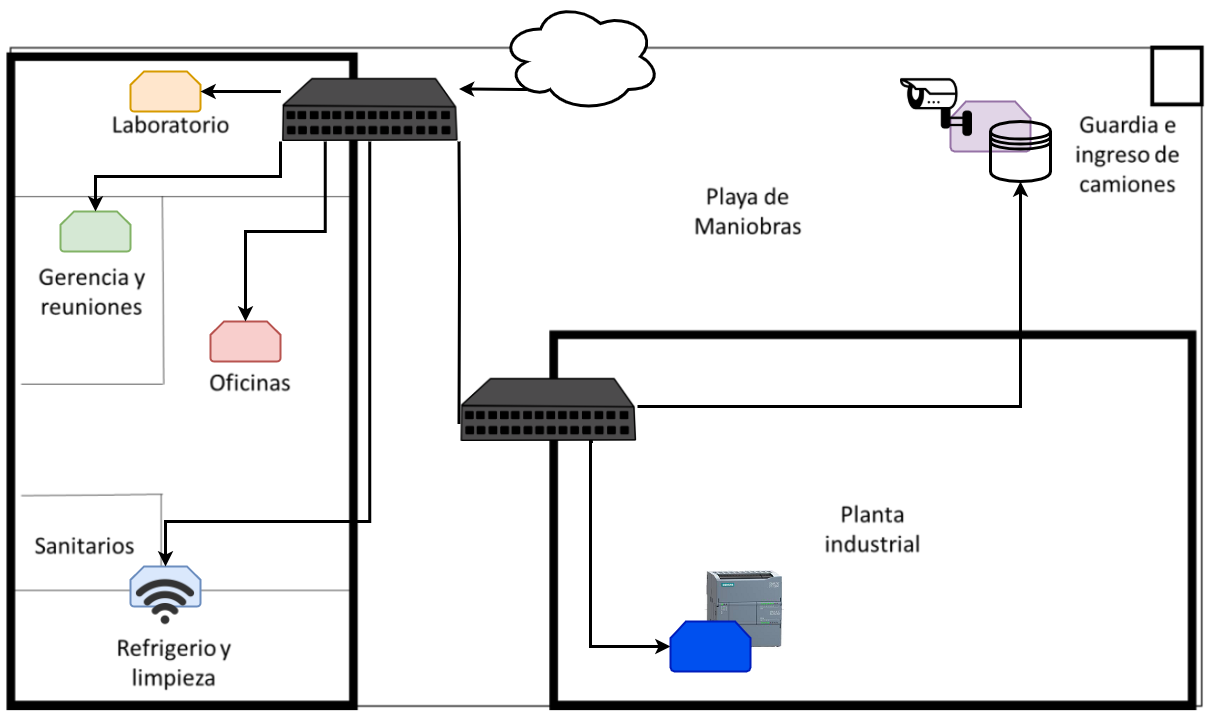
\includegraphics[width=\textwidth]{Figure/Planta_de_parque.png}
        \end{figure}
        

    \subsection{Parque industrial Rincón de los Sauces}

    Se utiliza un switch Cisco SF220-24-K9. Y se implementaran las siguientes VLAN's: 

    \begin{enumerate}
        \item Cámaras de seguridad: Al igual que en parque central se utilizara un dvr 
        \href{https://articulo.mercadolibre.com.ar/MLA-658974667-nvr-dvr-dahua-4-canales-penta-hdcvi-xvr-1a04-5-ch-5x1-qr-ps2-_JM#position=1&type=item&tracking_id=c1ba311d-e835-4420-9ba9-f01382834064}{\textit{Dahua 4 canales}} e ira conectado por un cable al switch principal.
        \item Oficinas: Cuentan con su propia VLAN con VPN.
        \item Instrumentos: Cuentan con una VLAN cableada con VPN.
        \item Refrigerio, limpieza y sanitarios: Red Wi-Fi sin VPN con access point tp-link. 
    \end{enumerate}

    \begin{figure}[H]
        \centering
        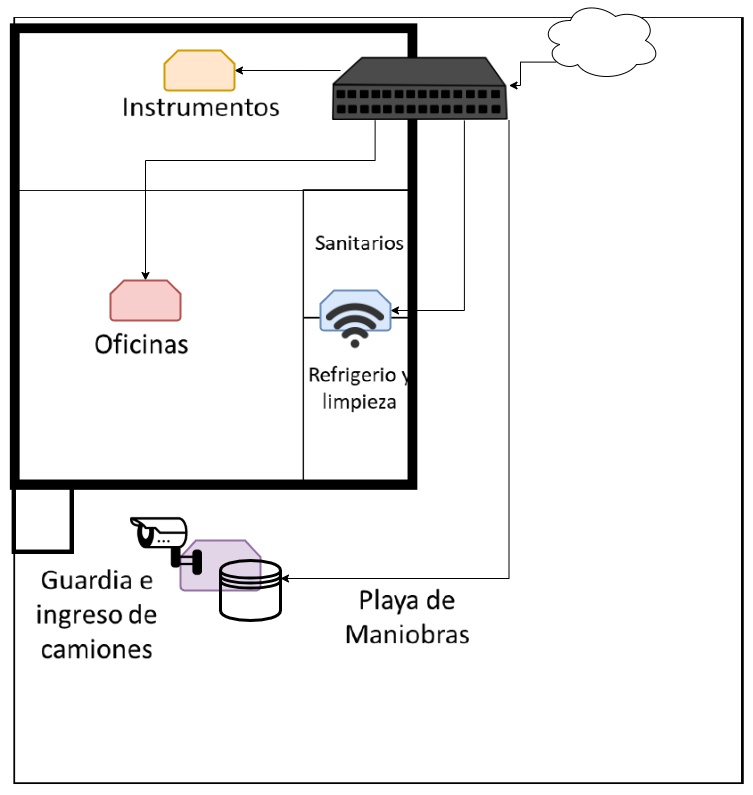
\includegraphics[width=0.6\textwidth]{Figure/Parque_Industrial.png}
    \end{figure}

 



    \subsection{Oficinas comerciales Neuquén}

    En esta oficina se utilizaran dos access point para garantizar las conexiones y no tener que invertir en cableado. Se utilizará un acces point 
    \href{https://www.mercadolibre.com.ar/access-point-interior-ubiquiti-networks-unifi-ac-lr-ap-uap-ac-lr-blanco-1-unidad/p/MLA7953376?pdp_filters=category:MLA1700#searchVariation=MLA7953376&position=1&type=product&tracking_id=933ff74a-93c5-4a58-9a31-9fe5a3c5746e}{\textit{Ubiquiti Unifi Uap-lr}}
    por cada piso.

    \subsection{Centro de logística Bahía Blanca}
    Se utiliza la misma idea de para las cámaras de seguridad de parque industrial y al ser pocas personas la conectividad será directamente del router/modem 
    del proveedor de internet. De esta forma se evita comprar un switch. 
    

    \section{Presupuesto}

    \begin{table}[H]
        \centering
        \begin{tabular}{|c|c|c|c|}
    \hline Nombre & Modelo & Cantidad & Precio [u$\$$d] \\ 
    \hline Servidor dedicado & Single Xeon quad-core & 1 & $128.75$ \\ 
    \hline Rastreador satelital & Galileo & - & $11.25$ \\
    \hline Switch Cisco & Sf220-24-k9 & 3 & $225$ \\
    \hline Dvr Dahua & DH XVR 1A08 & 1 & $100$ \\ 
    \hline Dvr Dahua & XVR 1A04 & 2 & $68.75$ \\ 
    \hline Access point tp-link & C80 & 2 & $71.25$ \\ 
    \hline Access point Ubiquiti & AC LR AP & 2 & $168.6$\\

    \rowcolor{LightYellow}
    \hline \multicolumn{3}{|c|}{Total} & $1520.95$\\
    \hline
    
\end{tabular}
        \caption{Presupuesto en dólares.}
    \end{table}

    \end{document}
